\chapter{O projeto do produto} 
\label{chap:projeto_do_produto} 

Existem diversos tipos de projetos necessários à implementação e funcionamento de uma empresa industrial. No presente capítulo será focado em demonstrar como o projeto do produto pode ser fornecido pela empresa. Essa atividade parte da etapa inicial (conceito, triagem do conceito, projeto preliminar, avaliação do projeto preliminar, construção de protótipos e projeto final do produto), passa pela documentação final resultante do projeto do produto até chegar na gestão do projeto de novos produtos. No final desta seção será mostrado como a \textit{SunBurn} utilizou destes conceitos para conceber o seu produto.

\section{Sec1} 
\label{sec:projeto_do_produto_sec1} 

Para conceber um projeto final de um produto é necessário que o projeto passe por diversas etapas fundamentais. Com isso, um fluxograma é formado como mostrado na Figura \ref{fig:projeto_produto}, mesmo que, na prática os projetistas avancem ou retrocedam pelas etapas. Serão descritas a seguir cada etapa deste processo na ordem em que geralmente ocorrem.

\begin{figure}[H]
  \centering
  \caption{Fluxograma das etapas do projeto do produto.}
  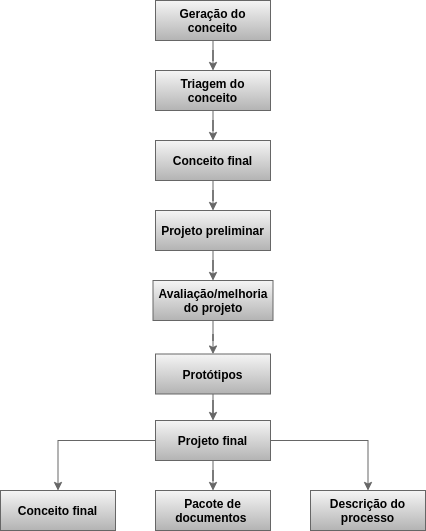
\includegraphics[width=1\textwidth]{images/projeto_produto.png}
  \caption*{Fonte: Adaptado \cite{slack2006administracao} }
  \label{fig:projeto_produto}
\end{figure}

\textbf{Geração do conceito:} É a primeira etapa para o desenvolvimento do projeto de um produto. É nesta fase que se elabora um resumo completo do conjunto de benefícios que o produto, quando fabricado, deverá proporcionar ao seu usuário, podendo ser ou não cliente direto da empresa. Tais benefícios devem corresponder às necessidades, desejos e expectativa do usuário, portanto, esta é uma atividade responsável pela equipe de \textit{marketing}, pois são eles que fazem a ponte entre o usuário e o pessoal operacional da empresa.  

\textbf{Triagem do conceito:} Nesta etapa ocorre uma avaliação entre as diversas alternativas de conceitos concebidas na etapa anterior. Esta avaliação, segundo \cite{slack2006administracao}, deve considerar a importância de cada solução elaborada, de modo que possam ser feitas escolhas entre elas. Cada opção é avaliada a partir de três categorias de critérios: a viabilidade - "quão difícil é o projeto?", a aceitabilidade - "ele vale a pena?" e a vulnerabilidade - "o que pode dar errado?".

\textbf{Conceito final:} Feita toda as avaliações da etapa anterior, obtém-se um conceito final do produto, que servirá de base para todo a parte de detalhamento técnico (forma, design, materiais, funcionalidades, resistência, segurança, durabilidade em uso e disponibilidade após a vida útil do produto). É importante lembrar que nesta etapa, ainda, não é apresentado os detalhes técnicos do produto, mas é indispensável para o referido detalhamento.

\textbf{Projeto preliminar:} Nesta etapa se inicia o detalhamento das informações de natureza técnica, fundamentais para a concepção do produto. Os documentos gerados nesta fase são, a princípio, os mesmos que farão parte da documentação final do projeto.

\textbf{Avaliação/melhoria do projeto:} O projeto do produto é uma atividade interativa, ou seja, está sujeita a sucessivas otimizações a medida em que evolui. Existem diversas técnicas ou ferramentas para a revisão e melhoria do projeto de um produto, dentre elas, destacam-se: o \ac{QFD}, engenharia de valor e os testes acelerados de resistência.

\textbf{Protótipos:} Antes das empresas colocar seu produto em produção regular, elas constroem exemplares iniciais do seu produto. O objetivo desta etapa é realizar testes e ensaios para observar o desempenho do protótipo em relação aos conceitos e projetos em fase de avaliações e melhorias.

\textbf{Projeto final:} A última etapa do processo consiste em elaborar um documento que contenha o conjunto de informações e especificações técnicas, que não deixem margem à dúvidas ou equívocos, para a produção do produto para o mercado. Segundo \cite{slack2006administracao}, a documentação final do projeto de um produto deve conter: o conceito final definitivo, "pacote de documentos do produto" (estrutura do produto, lista de materiais, especificações técnicas e seus componentes) e a descrição do processo de fabricação/montagem do produto (fluxograma). 


\section{Aplicação Prática} 
\label{sec:projeto_do_produto_aplicacao}